\begin{frame}{BLC1/2解析}
  \label{page:BLC}
  \centering
  \begin{tabular}{cccc}
    \begin{minipage}{0.1\hsize}
      BLC1
    \end{minipage}
    \begin{minipage}{0.3\hsize}
      \centering
      \begin{figure}
        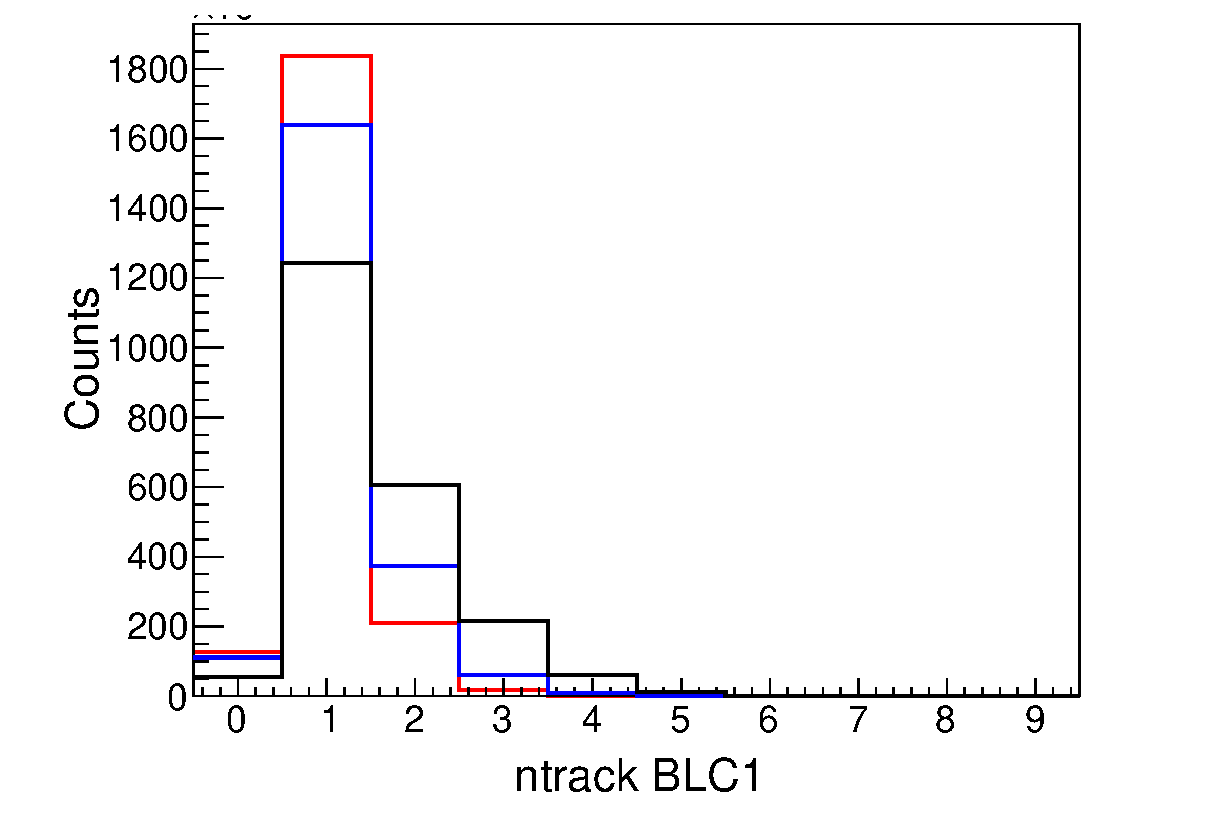
\includegraphics[width=3cm]{../pic/Run78/BL/nBLC1.eps}
      \end{figure}
    \end{minipage}
    \begin{minipage}{0.3\hsize}
      \centering
      \begin{figure}
        \includegraphics[width=3cm]{../pic/Run78/BL/BLC1_time.eps}
      \end{figure}
    \end{minipage}
    \begin{minipage}{0.3\hsize}
      \centering
      \begin{figure}
        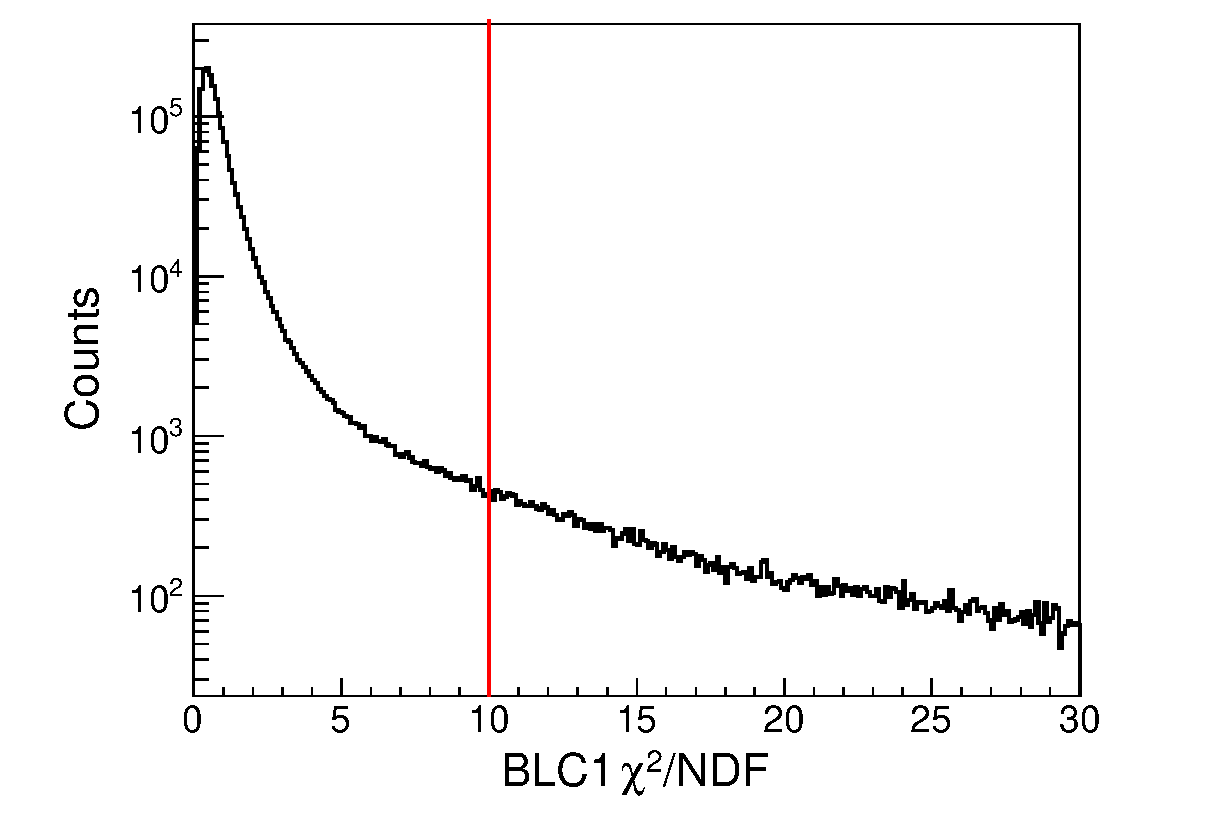
\includegraphics[width=3cm]{../pic/Run78/BL/BLC1_chi2.eps}
      \end{figure}
    \end{minipage}
  \end{tabular}

  \begin{tabular}{cccc}
    \begin{minipage}{0.1\hsize}
      BLC2
    \end{minipage}
    \begin{minipage}{0.3\hsize}
      \centering
      \begin{figure}
        \includegraphics[width=3cm]{../pic/Run78/BL/nBLC2.eps}
      \end{figure}
    \end{minipage}
    \begin{minipage}{0.3\hsize}
      \centering
      \begin{figure}
        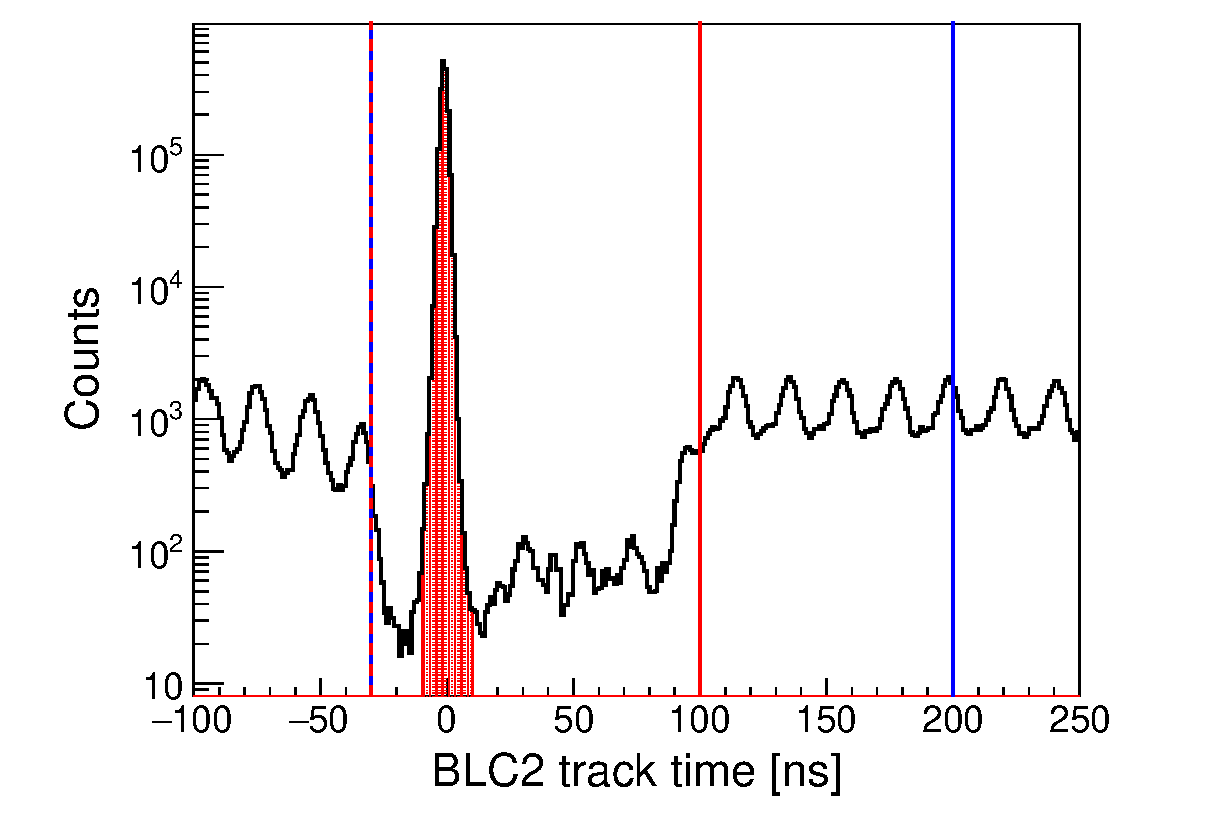
\includegraphics[width=3cm]{../pic/Run78/BL/BLC2_time.eps}
      \end{figure}
    \end{minipage}
    \begin{minipage}{0.3\hsize}
      \centering
      \begin{figure}
        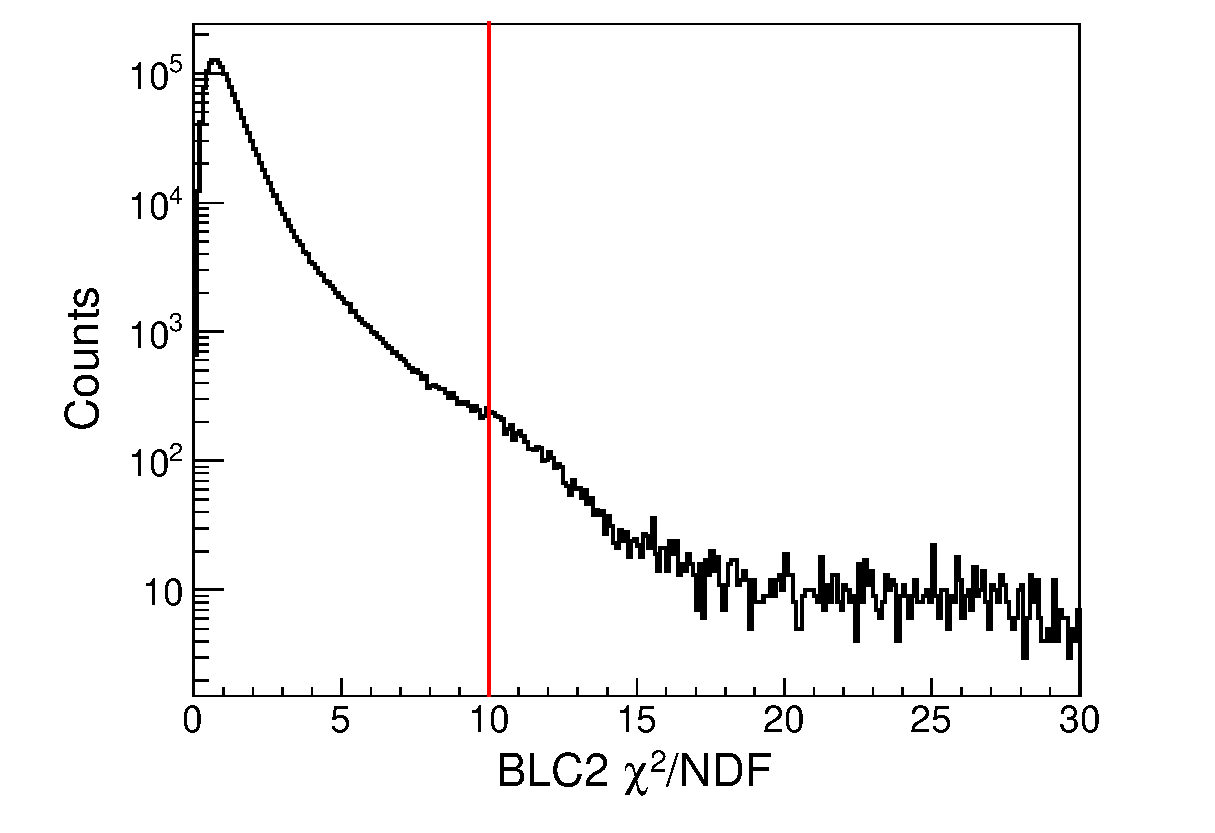
\includegraphics[width=3cm]{../pic/Run78/BL/BLC2_chi2.eps}
      \end{figure}
    \end{minipage}
  \end{tabular}

  \begin{tabular}{cccc}
    \begin{minipage}{0.1\hsize}
      \textcolor{white}{ ダミー }
    \end{minipage}
    \begin{minipage}{0.3\hsize}
      \centering
      \tiny
      トラックの数、黒線はすべて\\
      青は$-50 \sim 200$nsの時間窓\\
      赤は$-50 \sim 100$nsの時間窓\\
    \end{minipage}
    \begin{minipage}{0.3\hsize}
      \centering
      \tiny
      トラックの通過した時間\\
      0にビームに同期したピークが見える\\
      $-50 \sim 100$nsに1トラック\\
      それがビームに同期している(赤領域)であることを要求する
    \end{minipage}
    \begin{minipage}{0.3\hsize}
      \centering
      \tiny
      $\chi^2/NDF$分布、\\
      10以下(赤線)であるものを\\
      ビームとみなす。
    \end{minipage}
  \end{tabular}
\end{frame}
